\documentclass[11pt]{article}
\usepackage{myz310e-notes}
\hypersetup{pdftitle={Learning from data: tasks, representations and notation},pdfauthor={Emre Onur Kahya},pdfsubject={MYZ 310E Machine Learning in Physics, Fall 2026, lecture note 1 (week 1)}}

\begin{document}
\NoteTitle{1}{1}{Learning from data:\\ tasks, representations and notation}{Learning from data}{%
Machine learning replaces hand-written rules by functions estimated from examples. This note fixes the vocabulary
and notation used throughout the course: what a dataset is, how an observation becomes a vector, which kinds of
learning problems exist and how success is measured. Later notes refer back to Section~\ref{sec:notation}
(notation) and Table~\ref{tab:tasks} (tasks and losses) instead of repeating them.}

\section{Learning from examples}

Suppose we want a program that decides whether a photograph shows a horse. Writing the rules by hand --- four
legs, a mane, a long head, unless it is a donkey, unless the horse is lying down --- quickly becomes hopeless.
The machine-learning approach is different: collect many photographs labelled ``horse'' or ``not horse'' and let an
algorithm \emph{find} a function that maps images to labels. The principle is far more general than any single
application: the same algorithm, given different examples, learns to recognise galaxies, transcribe speech or
predict the energy of a particle shower.

\begin{keyidea}
Learning is not memorising. A table that stores every training image with its label answers perfectly on those
images and is useless on a new one. What we want is \emph{generalisation}: good predictions for cases never seen
during training. Note~4 makes this precise and shows how to measure it honestly.
\end{keyidea}

\begin{modern}{rules versus data}
The largest systems built today follow this principle at an enormous scale. A large language model is not given a
grammar of English or Turkish; it is trained to predict the next piece of text from the previous ones on trillions
of words, and grammar, facts and some reasoning skills emerge as by-products~\cite{vaswani2017,brown2020}. Image
classifiers trained on ImageNet's 1.28 million labelled photographs~\cite{russakovsky2015} replaced decades of
hand-designed vision pipelines.
\end{modern}

\begin{physics}{from cuts to classifiers}
Particle-physics analyses traditionally separated signal from background with hand-tuned \emph{cuts} on a few
observables (``transverse momentum above 25~GeV, invariant mass within 10~GeV of the $Z$ peak''). Today the same
decision is often made by a classifier trained on simulated events; for identifying boosted top quarks, for
example, learned taggers that read low-level detector information outperform the best hand-designed
variables~\cite{kasieczka2019}. The physics knowledge does not disappear --- it moves into the simulation, the
choice of inputs and the validation of the classifier.
\end{physics}

\section{Data and notation}\label{sec:notation}

\paragraph{Examples} An \emph{example} (observation, sample) is a pair $(\x, y)$. The \emph{input} $\x$ is a
vector of $d$ real numbers, $\x = (x_1, \dots, x_d)\T \in \R^d$, whose components are called \emph{features}. The
\emph{target} (label, desired output) $y$ is what we want to predict. A \emph{training set} of $n$ examples is
\[
  D_n = \{(\x_1, y_1), (\x_2, y_2), \dots, (\x_n, y_n)\}.
\]
Stacking the inputs as rows gives the \emph{design matrix} $X \in \R^{n \times d}$ whose $i$-th row is $\x_i\T$; the
targets form a vector $\vect{y} \in \R^n$ (or, for $m$ classes, a matrix of one-hot rows). Subscripts index
examples ($\x_i$), and when needed a bracket indexes features: $x_{i,j}$ or $\x_i[j]$ is feature $j$ of example $i$.
A \emph{predictor} is a function $f : \R^d \to \mathcal{Y}$; a new input whose target is unknown is a \emph{test
point}.

\paragraph{Problem size} Three numbers decide which algorithms are even feasible: the number of examples $n$, the
input dimension $d$ and the number of outputs (for classification, the number of classes $m$). Table~\ref{tab:size}
gives orders of magnitude.

\begin{table}[h]\centering\small
\caption{Typical problem sizes. The cost of most algorithms grows with $n$, $d$ and $m$ in very different ways.}
\label{tab:size}
\begin{tabular}{@{}llll@{}}\toprule
 & $n$ (examples) & $d$ (input dimension) & $m$ (classes) \\ \midrule
Iris flowers (1936) & 150 & 4 & 3 \\
Handwritten digits (MNIST) & 60\,000 & 784 (28$\times$28 pixels) & 10 \\
ImageNet classification & $1.28 \times 10^6$ & 150\,528 (224$\times$224$\times$3) & 1000 \\
Language-model pre-training & $10^{12}$--$10^{13}$ tokens & embedding size $\sim 10^3$--$10^4$ & vocabulary $\sim 10^5$ \\
Jet tagging at the LHC & $10^6$--$10^7$ simulated jets & $10^2$--$10^3$ constituents' features & 2--10 \\ \bottomrule
\end{tabular}
\end{table}

\paragraph{The i.i.d.\ assumption} We model each example $Z_i = (\X_i, Y_i)$ as a draw from an \emph{unknown}
joint distribution $P(\X, Y)$ --- ``nature'' or the experiment. Unless stated otherwise the examples are assumed
\emph{independent and identically distributed} (i.i.d.): every example comes from the same distribution, independently
of the others. Two consequences are used constantly: the order of the examples carries no information (shuffling the
dataset changes nothing), and a randomly chosen subset is a fair sample of the whole.

\begin{keyidea}[Not every dataset is i.i.d.]
Time series (tomorrow depends on today), grouped data (several images of the same galaxy or patient), data whose
distribution changes over time, and models trained on simulation but applied to real detector data (the
\emph{simulation-to-reality gap}) all violate the assumption. Methods that ignore this produce optimistic results;
Note~4 shows how to split such data correctly.
\end{keyidea}

\paragraph{Geometric picture} A dataset is a cloud of $n$ points in $\R^d$, each carrying a label. A test point is a
new location in that space, and learning means deciding what to predict \emph{everywhere} in $\R^d$, including in
regions where no training point lies. This picture --- points in a high-dimensional space --- underlies every method
in weeks~1--3, and its difficulties in large $d$ are the subject of Note~3.

\section{From raw observations to vectors}

Most learning algorithms of this course require each example to be a vector of fixed dimension $d$. How we build that
vector --- the \emph{representation} --- often matters more than the choice of algorithm.

\paragraph{Raw representations} A grey-scale image of $28 \times 28$ pixels becomes a vector of $d = 784$ intensities;
a colour image of $224 \times 224$ pixels has $d = 150\,528$. A waveform or a detector read-out can be used as is.
Raw vectors are easy to produce but awkward: a shift of the object by one pixel changes almost every coordinate.

\paragraph{Hand-crafted features} Domain experts design a few informative quantities. For documents, the
\emph{bag of words} counts how often each word of a vocabulary occurs, so ``the cat jumped'' becomes a long vector of
zeros with three ones; it forgets word order, so ``dog bites man'' and ``man bites dog'' get the same vector. In
vision, histograms of oriented gradients and SIFT descriptors~\cite{dalal2005,lowe2004} summarise local edge
directions. In physics, features are often physical observables: invariant masses, transverse momenta, or
jet-substructure variables built from the theory of QCD.

\paragraph{Learned representations} Deep networks learn the features themselves from raw inputs, layer by layer, from
edges to parts to objects. The learned intermediate vectors --- \emph{embeddings} --- are now reused far beyond the task
they were trained for: a word or token is mapped to a vector of a few hundred to a few thousand dimensions (768 in
BERT-base~\cite{devlin2019}), and models such as CLIP map images and captions into a \emph{shared} space where
matching pairs are close~\cite{radford2021}. For text, the raw input is first split into \emph{tokens} from a
vocabulary of $10^4$--$10^5$ pieces, and each token is looked up in an embedding table.

\begin{modern}{representations as a product}
A common recipe in 2026 is to take a large pre-trained model, keep it frozen, and train only a simple classifier
--- or even a nearest-neighbour rule (Note~5) --- on its embeddings. The algorithms of weeks~1--3 are therefore not
museum pieces: they are exactly what is applied on top of modern representations.
\end{modern}

\section{Families of learning problems}

\paragraph{Supervised learning} predicts a target $y$ from an input $\x$. In \emph{classification} $y$ is a category
(binary, $y \in \{0,1\}$ or $\{-1,+1\}$; or multiclass, $y \in \{1, \dots, m\}$). In \emph{regression} $y$ is a real
number or a vector of real numbers.

\paragraph{Unsupervised learning} has no explicit target. \emph{Density estimation} models the distribution $p(\x)$
of the inputs; \emph{clustering} groups similar examples; \emph{dimensionality reduction} finds a few coordinates that
describe the data (for visualisation or compression); \emph{representation learning} builds useful features.

\paragraph{Between the two} \emph{Semi-supervised} learning uses a few labelled and many unlabelled examples.
\emph{Self-supervised} learning manufactures targets from the data itself: predict the next token of a text, a masked
patch of an image, or which caption belongs to which image. Next-token prediction is, formally, multiclass
classification with $m$ equal to the vocabulary size, repeated at every position of every text --- which is why the
simple losses below also drive the largest models.

\paragraph{Reinforcement learning} An agent chooses actions in an environment to maximise a cumulative reward; it is
used, for example, to fine-tune language models from human preference judgements~\cite{ouyang2022}. It is outside
the scope of this course.

\begin{figure}[h]\centering
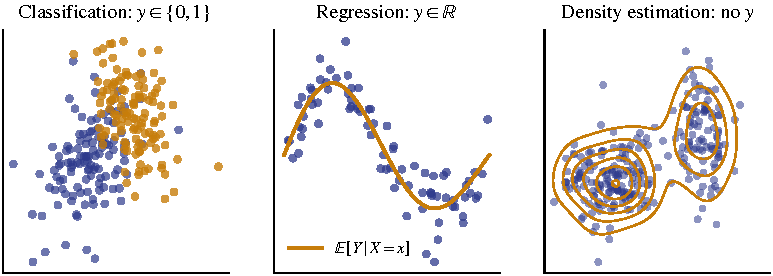
\includegraphics[width=\linewidth]{figures/tasks}
\caption{Three tasks. Left: classify events into signal (amber) and background (indigo) from two observables. Middle: regression;
the curve is the conditional mean $\E[Y \mid X = x]$ that a good regressor approximates. Right: density estimation;
contours of an estimate of $p(\x)$ (Note~5 explains how it was computed).}
\label{fig:tasks}
\end{figure}

\begin{table}[h]\centering\small
\caption{The three classic problems. This table is the reference for the rest of the course.}
\label{tab:tasks}
\renewcommand{\arraystretch}{1.25}
\begin{tabular}{@{}L{0.17\linewidth}L{0.16\linewidth}L{0.36\linewidth}L{0.23\linewidth}@{}}\toprule
 & Target & What $f(\x)$ should be & Typical loss $L$ \\ \midrule
Classification & $y \in \{1, \dots, m\}$ & the most probable class, or the vector of probabilities $P(Y = k \mid \X = \x)$ & error $\ind{f(\x) \neq y}$ \\
Regression & $y \in \R$ & the conditional mean $\E[Y \mid \X = \x]$ & squared error $(f(\x) - y)^2$ \\
Density estimation & none & the density $p(\x)$ & negative log-likelihood $-\log f(\x)$ \\ \bottomrule
\end{tabular}
\end{table}

Why these targets? For squared error, conditioning on $\X = \x$ and writing $\mu(\x) = \E[Y \mid \X = \x]$,
\[
  \E\big[(f(\x) - Y)^2 \mid \X = \x\big] = \big(f(\x) - \mu(\x)\big)^2 + \Var(Y \mid \X = \x),
\]
so the best possible prediction is $\mu(\x)$, and the remaining $\Var(Y \mid \X = \x)$ is noise that no predictor can
remove. Similarly, the expected classification error at $\x$ is $1 - P(Y = f(\x) \mid \X = \x)$, minimised by the most
probable class (Exercise~E3). The irreducible error that remains is called the \emph{Bayes error}.

\paragraph{One dataset, several tasks} The task is a choice of the analyst, not a property of the data. From the same
galaxy survey one can classify morphology (spiral or elliptical), regress the redshift from the measured colours
(``photometric redshifts''), or estimate the density of objects in colour space and flag the rare ones that fall in
low-density regions --- a standard route to discovering unusual objects.

\section{Anatomy of a machine-learning project}\label{sec:workflow}

\begin{enumerate}
\item \textbf{Formulate.} Which task of Table~\ref{tab:tasks} is it? Which loss reflects what you actually care about
(a missed signal event and a false alarm rarely cost the same)?
\item \textbf{Understand the data.} How many examples, what is one example, how were labels obtained (by experts,
by simulation, by an older algorithm?), and what is the unit of independence?
\item \textbf{Split first.} Set aside validation and test data \emph{before} looking for patterns (Note~4).
\item \textbf{Pre-process using training data only.} Scaling constants, vocabularies and feature selections are part
of the model; computing them on all the data leaks information from the test set.
\item \textbf{Start simple.} A constant predictor, a linear model or a nearest-neighbour rule gives a baseline. Debug on
low-dimensional problems where the data and the decision boundary can be plotted and training takes seconds.
\item \textbf{Evaluate out of sample}, compare models fairly and report uncertainty (Note~4).
\item \textbf{Deploy and monitor.} The data distribution can drift after deployment.
\end{enumerate}

\begin{modern}{leakage in published science}
A survey of machine-learning-based science found data leakage --- for example pre-processing on the full dataset,
duplicates across splits, or features that encode the label --- in hundreds of published papers across seventeen
fields, often turning a useless model into an apparently excellent one~\cite{kapoor2023}. Steps 3 and 4 above are the
cheapest insurance against it. Documenting how a dataset was collected (``datasheets for datasets''~\cite{gebru2021})
helps others detect such problems.
\end{modern}

\section{A vector toolkit}\label{sec:vectors}

For $\vect{a}, \vect{b} \in \R^d$ the \emph{inner product} is $\vect{a}\T\vect{b} = \sum_{j=1}^d a_j b_j$. The
\emph{$L_p$ norm} is $\norm{\vect{a}}_p = \big(\sum_j |a_j|^p\big)^{1/p}$ for $p \ge 1$; $p = 2$ gives the Euclidean
norm $\norm{\vect{a}} = \sqrt{\vect{a}\T\vect{a}}$, $p = 1$ the sum of absolute values and $p \to \infty$ the largest
absolute value. The Euclidean distance is $\norm{\vect{a} - \vect{b}}$, and the \emph{cosine similarity}
$\cos(\vect{a},\vect{b}) = \vect{a}\T\vect{b} / (\norm{\vect{a}}\,\norm{\vect{b}})$ compares directions only --- the
standard way to compare embeddings.

\paragraph{Distances in bulk} Many methods need the distances between $q$ query points (rows of $Q \in \R^{q \times
d}$) and $n$ data points (rows of $X$). Expanding the square,
\[
  \norm{\vect{a} - \vect{b}}^2 = \norm{\vect{a}}^2 + \norm{\vect{b}}^2 - 2\,\vect{a}\T\vect{b},
\]
so the whole $q \times n$ matrix of squared distances is two vectors of squared norms plus the single matrix product
$-2\,QX\T$. Matrix products are what modern hardware does best; the loop over pairs disappears.

\begin{verbatim}
import numpy as np
def sq_distances(Q, X):          # Q: (q, d), X: (n, d)
    D = (Q**2).sum(1)[:, None] + (X**2).sum(1)[None, :] - 2 * Q @ X.T
    return np.maximum(D, 0)      # round-off can make tiny values negative
\end{verbatim}

The cost is $O(qnd)$ operations either way; the gain is that they run as one optimised matrix multiplication.
Note~5 builds the nearest-neighbour algorithm on this function.

\begin{keyidea}[Summary]
An example is a pair $(\x, y)$ with $\x \in \R^d$; a dataset is $n$ such pairs, assumed i.i.d.\ from an unknown
$P(\X, Y)$. Representations range from raw measurements through hand-crafted features to learned embeddings. Tasks
are supervised (classification, regression), unsupervised (density estimation and others) or in between
(self-supervised); each comes with a natural target and loss (Table~\ref{tab:tasks}). The goal is always
generalisation to new data.
\end{keyidea}

\begin{exercises}
\item What is the input dimension $d$ of (a) a $64 \times 64$ colour image, (b) a one-hot encoding of a word from a
vocabulary of 50\,000 words, (c) a sequence of 128 tokens, each embedded in $\R^{768}$, flattened into one vector?
\item Prove the decomposition of the conditional expected squared error in Section~4 and conclude that $\E[Y\mid\X=\x]$
is the best regressor.
\item Show that the expected classification error at $\x$ equals $1 - P(Y = f(\x) \mid \X = \x)$ and is minimised by
$f(\x) = \argmax_k P(Y = k \mid \X = \x)$.
\item Is the i.i.d.\ assumption reasonable for a random train/test split of (a) collision events recorded in one run
of an experiment, (b) consecutive frames of the same video, (c) data from 2024 used to predict 2025, (d) galaxy images
where each galaxy was photographed several times? For each ``no'', propose a better split.
\item Implement \texttt{sq\_distances}, check it against a double loop on small random matrices, and compare running
times for $q = 1000$, $n = 10\,000$, $d = 128$.
\item Give two sentences with identical bag-of-words vectors and different meanings. Which kind of representation
of Section~3 can tell them apart, and why?
\end{exercises}

\paragraph{Further reading} Bishop~\cite{bishop2006}, chapter~1; Murphy~\cite{murphy2022}, chapter~1; for applications
across physics, the review by Carleo \emph{et al.}~\cite{carleo2019}.

\begin{thebibliography}{99}\small
\bibitem{bishop2006} C.~M. Bishop, \emph{Pattern Recognition and Machine Learning}, Springer (2006).
\bibitem{brown2020} T.~Brown \emph{et al.}, Language models are few-shot learners, \emph{NeurIPS} (2020).
\bibitem{carleo2019} G.~Carleo \emph{et al.}, Machine learning and the physical sciences, \emph{Rev.\ Mod.\ Phys.}\ 91, 045002 (2019).
\bibitem{dalal2005} N.~Dalal and B.~Triggs, Histograms of oriented gradients for human detection, \emph{CVPR} (2005).
\bibitem{devlin2019} J.~Devlin \emph{et al.}, BERT: pre-training of deep bidirectional transformers for language understanding, \emph{NAACL} (2019).
\bibitem{gebru2021} T.~Gebru \emph{et al.}, Datasheets for datasets, \emph{Commun.\ ACM} 64(12), 86--92 (2021).
\bibitem{kapoor2023} S.~Kapoor and A.~Narayanan, Leakage and the reproducibility crisis in machine-learning-based science, \emph{Patterns} 4(9), 100804 (2023).
\bibitem{kasieczka2019} G.~Kasieczka \emph{et al.}, The machine learning landscape of top taggers, \emph{SciPost Phys.}\ 7, 014 (2019).
\bibitem{lowe2004} D.~G. Lowe, Distinctive image features from scale-invariant keypoints, \emph{Int.\ J.\ Comput.\ Vis.}\ 60, 91--110 (2004).
\bibitem{murphy2022} K.~P. Murphy, \emph{Probabilistic Machine Learning: An Introduction}, MIT Press (2022).
\bibitem{ouyang2022} L.~Ouyang \emph{et al.}, Training language models to follow instructions with human feedback, \emph{NeurIPS} (2022).
\bibitem{radford2021} A.~Radford \emph{et al.}, Learning transferable visual models from natural language supervision, \emph{ICML} (2021).
\bibitem{russakovsky2015} O.~Russakovsky \emph{et al.}, ImageNet large scale visual recognition challenge, \emph{Int.\ J.\ Comput.\ Vis.}\ 115, 211--252 (2015).
\bibitem{vaswani2017} A.~Vaswani \emph{et al.}, Attention is all you need, \emph{NeurIPS} (2017).
\end{thebibliography}

\SourceNote
\end{document}
